\documentclass[oneside,a4paper,11pt]{report}
\usepackage{fullpage}

\usepackage{../../info/packages}
\usepackage{../../info/nomenclature}

\setlength{\cellspacetoplimit}{3pt}
\setlength{\cellspacebottomlimit}{3pt}

\title{Numerical Methods\thanks{Disclaimer: a large chunk of the work in this document is not original; instead, parts of this document are personal notes obtained from the following books: Lomax, Pulliam, Zing; Larsson, Thomee; Hirsch; Leveque; Blazek; Laney; Moin.}}
\date{\today}
\author{Alejandro Campos}

\begin{document}
\maketitle
\tableofcontents

%##########################################################################
\part{Introductory Concepts}
%##########################################################################
\begin{itemize}
\item Analytical solution $u$ satisfies
\begin{equation}
D(u) = Au - f = 0\quad \text{in } \Omega,
\label{pde}
\end{equation}
where $A$ is the differential operator.

\item Discrete numerical solution $U_j$ satisfies 
\begin{equation}
D_h(U^n_j) = 0 \quad \text{for all } n, j ,
\end{equation}
where $D_h$ is the discrete operator for $D$.

\item Continuous numerical solution $v$ satisfies
\begin{equation}
D_hv = 0 \quad \text{in } \Omega,
\label{npde}
\end{equation}
Thus, $v(t_n, x_j) = U^n_j$ for all $n, j$.

\item Local truncation error 
\begin{equation}
l^{n+1}_j = u(t_{n+1}, x_j) - U^{n+1}_j,
\end{equation}
given that $U^n_j = u(t_n, x_j)$ for all $j$. 

\item Global truncation error
\begin{equation}
e^{n+1}_j = u(t_{n+1}, x_j) - U^{n+1}_j,
\end{equation}
given that $U^0_j = u(t_0, x_j)$ for all $j$.

\item Truncation error $\tau$: difference between the discrete and analytical equations when applied to a given continuous function $g$
\begin{equation}
\tau = D_hg - Dg.
\label{trunc}
\end{equation}

The truncation error allows us to compute global truncation errors. Also, consider the truncation error for the analytical solution, that is, $\tau = D_hu - Du$. Using equation (\ref{pde}), one obtains that $u$ is also the solution to $D_hu = \tau$. This means that the \textbf{analytical solution satisfies the numerical equation but with an additional source term equal to $\tau$}. Conversely, consider the truncation error for the function $v$, $\tau = D_hv - Dv$. Using equation (\ref{npde}), one obtains that $v$ is also a solution to $Dv = \tau$. This means that the \textbf{numerical solution satisfies the analytical equation but with an additional source term equal to $\tau$}.

\item Order of accuracy $r$ defined by $\tau^n = \mathcal{O}(\Delta t^r)$ as $\Delta t \to 0$ for ODE's and $\tau^n = \mathcal{O}(\Delta x^r)$ as $\Delta x \to 0$ for PDE's, where $\Delta t$ is related to $\Delta x$.

\end{itemize}

%##########################################################################
\part{Numerical Solution of ODE's}
%##########################################################################

%----------------------------------------------------------------------------------------------------------------------------
\chapter{List of time integrators}
%----------------------------------------------------------------------------------------------------------------------------
Consider the IVP for $u=u(t)$
\begin{equation}
\label{ode}
\frac{du}{dt} = f(t, u) \quad \text{in } (0,\infty)
\end{equation}
with initial condition $u(0) = u^0$. We will discretize time into a set of finite values $t^n$, and express the numerical solution at a given time $t^n$ as $U^n$. 

%----------------------------------------------------------------------------------------------------------------------------
\section{Explicit}
%----------------------------------------------------------------------------------------------------------------------------
\begin{itemize}

\item Explicit Euler method (Forward Euler method)
\begin{equation}
u^{n+1} = u^n + \Delta t f(t_n, u^n) \qquad \text{1\textsuperscript{st} O.A.}
\end{equation}

\item Explicit Midpoint (Modified Euler, 2\textsuperscript{nd} order RK)
\begin{align}
    u^{n+1/2} &= u^n + \frac{\Delta t}{2} f(t_n, u^n) \nonumber \\
    u^{n+1}   &= u^n + \Delta t f(t_{n+1/2}, u^{n+1/2})
\end{align}

\end{itemize}

%----------------------------------------------------------------------------------------------------------------------------
\section{Implicit}
%----------------------------------------------------------------------------------------------------------------------------
\begin{itemize}

\item Implicit Euler (Backward Euler)
\begin{equation}
u^{n+1} = u^n + \Delta t f(t_{n+1}, u^{n+1}) \qquad \text{1\textsuperscript{st} O.A.}
\end{equation}

\item Implicit Trapezoidal (Crank-Nicholson)
\begin{equation}
u^{n+1} = u^n + \frac{\Delta t}{2} [ f(t_n, u^n) + f(t_{n+1}, u^{n+1}) ] \qquad \text{2\textsuperscript{nd} O.A.}
\end{equation}

\item Implicit Midpoint
\begin{equation}
    u^{n+1} = u^n + \Delta t f\left (t_{n+1/2}, \frac{1}{2} \left (u^n + u^{n+1} \right ) \right )
\end{equation}

\end{itemize}

%----------------------------------------------------------------------------------------------------------------------------
\section{Predictor-Corrector}
%----------------------------------------------------------------------------------------------------------------------------
\begin{itemize}

\item Heun's (Explicit Trapezoidal, Improved Euler)
\begin{align}
\tilde{u}^{n+1} &= u^n + \Delta t f(t_n, u^n) \nonumber \\
u^{n+1}   &= u^n + \frac{\Delta t}{2} [ f(t_n, u^n) + f(t_{n+1}, \tilde{u}^{n+1}) ] \quad \text{2 \textsuperscript{nd} O.A.}
\end{align}

\end{itemize}

%----------------------------------------------------------------------------------------------------------------------------
\section{Runge-Kutta}
%----------------------------------------------------------------------------------------------------------------------------
\begin{itemize}
\item 4\textsuperscript{th} order Runge-Kutta
\begin{align}
k_1 &= f(t_n, u^n) \nonumber \\
k_2 & = f(t_{n+1/2}, u^n + \frac{\Delta t}{2} k_1) \nonumber \\
k_3 & = f(t_{n+1/2}, u^n + \frac{\Delta t}{2} k_2) \nonumber \\
k_4 & = f(t_n, u^n + \Delta t k_3) \nonumber \\
u^{n+1} &= u^n + \frac{\Delta t}{6} (k_1 + 2k_2 + 2k_3 + k_4)
\end{align}
\end{itemize}

%----------------------------------------------------------------------------------------------------------------------------
\section{Multi-Step}
%----------------------------------------------------------------------------------------------------------------------------
\begin{itemize}
\item Leapfrog: consider the system of equations for $x=x(t)$ and $v=v(t)$
\begin{equation}
    \frac{dx}{dt} = v \qquad \frac{dv}{dt} = f(x).
\end{equation}
The Leapfrog method is a staggered scheme defined as follows
\begin{align}
    v^{n+1/2} &= v^{n-1/2} + f(x^n) \Delta t \\
    x^{n+1} &= x^{n} + v^{n+1/2} \Delta t
\end{align}

\item Adams-Bashforth
\end{itemize}

%----------------------------------------------------------------------------------------------------------------------------
\chapter{Solving non-linear equations}
%----------------------------------------------------------------------------------------------------------------------------
The implicit schemes result in non-linear equations that require some sort of non-linear solver. For this chapter, we'll assume the governing ODE is
\begin{equation}
\label{eq:time_stepping_ode}
    \frac{du}{dt} = f(u) \qquad \text{in }(0,\infty),
\end{equation}
or, for a system of equations,
\begin{equation}
\label{eq:time_stepping_ode_system}
    \frac{d\uvec}{dt} = \fvec(\uvec) \qquad \text{in }(0,\infty).
\end{equation}

%----------------------------------------------------------------------------------------------------------------------------
\section{Newton's method}
%----------------------------------------------------------------------------------------------------------------------------
The Euler scheme requires finding $u^{n+1}$ so that the following is satisfied 
\begin{equation}
    u^{n+1} = u^n + \Delta t f(u^{n+1}).
\end{equation}
That is, we need to find the root of the nonlinear equation 
\begin{equation}
\label{eq:backward_euler_root}
    g(x) = x - u^n - \Delta t f(x).
\end{equation}
Newton's method finds the root of a non-linear equation $g(x)$ by iterating through $m$ as follows
\begin{equation}
    x^{m+1}=x^m - \frac{g(x^m)}{g'(x^m)}.
\end{equation}
Applying Newton's method to \cref{eq:backward_euler_root}, we have
\begin{equation}
\label{eq:backward_euler_newtons_method_scalar}
    x^{m+1} = x^m - \frac{x^m - u^n - \Delta t f(x^m)}{1 - \Delta t f'(x^m)},
\end{equation}
The initial value for the non-linear solver is $x^0 = u^n$. Thus, using the above, $u^{n+1}$ is approximated by $x^m$ as $m\to\infty$. Note that this is only one example of what is referred to as a fixed-point iteration. There are other fixed-point-iteration methods that can be used to solve \cref{eq:backward_euler_root} that are not Newton's method.

As a side note, let's assume $u^{n+1}$ is approximated sufficiently well by $x^1$, that is, only one Newton iteration is needed. Then we have
\begin{equation}
    u^{n+1} = u^n + \frac{\Delta t f(u^n)}{1 - \Delta t f'(u^n)}, 
\end{equation}
which we re-write as
\begin{equation}
\label{eq:backward_euler_pseudotime_stepping_scalar}
    \left ( \frac{1}{\Delta t} - f'(u^n) \right ) \Delta u = f(u^n),
\end{equation}
where $\Delta u = u^{n+1} - u^n$. The above is the approximation that gets used for pseudo-time stepping, so that the Backward Euler scheme can converge to the steady state solution as one iterates through $n$.

To solve for the root of a system of non-linear equations $\gvec(\xvec)$, Newton's method is as follows
\begin{equation}
    \xvec^{m+1} = \xvec^m - \Jvec^{-1}(\xvec^m) \gvec(\xvec^m). 
\end{equation}
In the above, $\Jvec^{-1}(\xvec)$ is the inverse of the Jacobian matrix $\Jvec(\xvec)$, which is given by
\begin{equation}
    \Jvec(\xvec) = \frac{\partial \gvec(\xvec)}{\partial \xvec} = \begin{pmatrix} 
    \frac{\partial g_1(\xvec)}{\partial x_1} & \frac{\partial g_1(\xvec)}{\partial x_2} & \dots \\
    \frac{\partial g_2(\xvec)}{\partial x_1} & \frac{\partial g_2(\xvec)}{\partial x_2} & \\
    \vdots &        & \ddots
    \end{pmatrix}.
\end{equation}
For the backward Euler scheme, the equivalent of \cref{eq:backward_euler_newtons_method_scalar} would be
\begin{equation}
\label{eq:backward_euler_newtons_method_system}
    \xvec^{m+1} = \xvec^m - \left ( \Ivec - \Delta t \left . \frac{\partial \fvec(\xvec)}{\partial \xvec} \right |_{\xvec = \xvec^m} \right )^{-1} \left ( \xvec^m - \uvec^n - \Delta t \fvec(\xvec^m) \right ),
\end{equation}
and the equivalent of \cref{eq:backward_euler_pseudotime_stepping_scalar} would be
\begin{equation}
\label{eq:backward_euler_pseudotime_stepping_system}
    \left ( \frac{\Ivec}{\Delta t} - \left . \frac{\partial \fvec(\xvec)}{\partial \xvec} \right |_{\xvec = \uvec^n} \right ) \Delta \uvec = \fvec(\uvec^n),
\end{equation}
where $\Delta \uvec = \uvec^{n+1} - \uvec^n$.


%##########################################################################
\part{Finite Difference for PDE's}
%##########################################################################

%----------------------------------------------------------------------------------------------------------------------------
\chapter{Introduction}
%----------------------------------------------------------------------------------------------------------------------------
%---------------------------------------------------------------
\section{Finite difference formulas}
%---------------------------------------------------------------
\begin{center}
\begin{tabular}{|c|c|c|c|}
\hline
Forward & Backward & Central & Central (2nd order)\\
\hline
\parbox{3cm}{\[\partial U_j = \frac{U_{j+1} - U_{j}}{h}\]} &
\parbox{3cm}{\[\bar{\partial} U_j = \frac{U_{j} - U_{j-1}}{h}\]} & 
\parbox{4cm}{\[\hat{\partial} U_j = \frac{U_{j+1} - U_{j-1}}{2h}\]} &
\parbox{5cm}{\[\partial \bar{\partial} U_j = \frac{U_{j+1} - 2U_j + U_{j-1}}{h^2}\]}\\
\hline
\end{tabular}
\end{center}

%---------------------------------------------------------------
\section{Fourier analysis}
%---------------------------------------------------------------
This analysis is based on a test function that is periodic and thus has the following form
\begin{equation}
    u(x) = \sum_{n = -\infty}^{n=\infty} \hat{u}_n e^{i \kappa_n x}.
\end{equation}
We are interested in using the different numerical methods to compute the resulting approximate derivatives of the generic mode $e^{i \kappa x}$. We note that one can then combine the approximate derivatives of all the modes to obtain the approximate derivative of our test function u.

The analytically derivative of our generic mode $e^{i\kappa x}$ is $i\kappa e^{i\kappa x}$. We now assume that the approximate derivatives at a point $x_j$ obtained using numerical schemes will be of the form $i\kappa^* e^{i\kappa x_j}$, where $\kappa^*$ is a modified wave number. The closer $\kappa^*$ is to $\kappa$ the higher the accuracy of the numerical scheme. For example, for the central first order scheme 
\begin{equation}
\delta U_j = \frac{ U_{j+1} - U_{j-1} }{ 2h }
\end{equation}
we have
\begin{equation}
    i\kappa^*e^{i\kappa x_j} = \frac{ e^{i\kappa (x_j+h) } - e^{ i \kappa (x_j-h)  } }{2h}
\end{equation}
which leads to
\begin{equation}
    \kappa^* = \frac{ \sin \kappa h }{h}.
\end{equation}

For the sixth-order compact scheme
\begin{equation}
    \alpha \delta U_{j-1} + \delta U_j + \alpha \delta U_{j+1} = \frac{a}{2h} \left( U_{j+1} - U_{j-1} \right) + \frac{b}{4h} \left ( U_{j+2} - U_{j-2} \right)
\end{equation}
we have
\begin{equation}
    \alpha i \kappa^* e^{i \kappa (x_j -h) } + i\kappa^* e^{i \kappa x_j} + \alpha i \kappa^* e^{i \kappa (x_j + h)} = \frac{a}{2h} \left [ e^{i \kappa (x_j+h) } - e^{ i \kappa (x_j-h) } \right ] + \frac{b}{2h} \left [ e^{i \kappa (x_j+2h) } - e^{ i \kappa (x_j-2h) } \right ]
\end{equation}
which leads to
\begin{equation}
    \kappa^* = \frac{ \frac{a}{h} \sin \kappa h + \frac{b}{2h} \sin 2\kappa h}{1 + 2\alpha \cos \kappa h}.
\end{equation}

A spectral method, on the other hand, will explicitly express the derivative of a mode as $i \kappa e^{i \kappa x_j}$, up to the last mode $\kappa = \frac{2 \pi}{L} \frac{N}{2}$, and will not be able to capture higher modes. Thus,
\begin{equation}
    \kappa^* = \begin{cases} \kappa \quad \text{for } \frac{2 \pi}{L} \left (-\frac{N}{2} +1 \right ) \le \kappa \le \frac{2 \pi}{L} \frac{N}{2} \\ 0 \quad \text{o.w.} \end{cases}
\end{equation}

%----------------------------------------------------------------------------------------------------------------------------
\chapter{Elliptic}
%----------------------------------------------------------------------------------------------------------------------------
Define the following norm: $|U|_S = \max_{x_j \in S}|U_j|$.\\
For $Au = -au''+cu=f$ in $\Omega=(0,1)$, where $a(x)>0$ and $c(x)\ge0$, with boundary conditions $u(0) = U_0$ and $u(1) = U_m$, and $A_h = -a_j\partial\bar{\partial}U_j + c_jU_j$:
\begin{itemize}
\item \textbf{Lemma 4.2} $$|U|_{\bar{\Omega}} \le \max\{|U_0|,|U_M|\} + C|A_hU|_{\Omega}$$

\item \textbf{Theorem 4.1} The error bound follows,
$$|U-u|_\Omega \le Ch^2||u||_C^4$$
\end{itemize}
For $Au = -\Delta u=f$ in $\Omega= (0,1)\times(0,1)$, with boundary doncitions $u=0$ in $\Gamma$, and $A_h = -\Delta_h = -\partial_1\bar{\partial_1}U_j - \partial_2\bar{\partial_2}U_j$:
\begin{itemize}
\item \textbf{Lemma 4.4} $$|U|_{\bar{\Omega}} \le |U|_\Gamma + C|\Delta_hU|_\Omega$$

\item \textbf{Theorem 4.2} The error bound follows,
$$|U-u|_\Omega \le Ch^2||u||_C^4$$
\end{itemize}

%----------------------------------------------------------------------------------------------------------------------------
\chapter{Parabolic}
%----------------------------------------------------------------------------------------------------------------------------
For $u_t = u_{xx}$ in $\mathbf{R}\times\mathbf{R_+}$, with initial condition $u(\cdot,0) = v$ in $\mathbf{R}$.
\begin{itemize}
\item Each scheme can be associated with its discrete solution operator $E_k$, defined in either of the following two ways, where $U^n_{j}$ is defined only at mesh points, and $u^n(x)$ is the corresponding numerical solution defined over all space,
$$U_j^{n+1} = (E_kU^n)_j = \sum_p a_pU_{j-p}^n$$
$$u^{n+1}(x) = (E_ku^n)(x) = \sum_p a_pu^n(x-x_p)$$

\item Repeated application yields $U^n_j = (E_k^nV)_j$ or $u^n(x) = (E_k^nv)(x)$, where $V_i$ and $v(x)$ are the initial conditions, specified at mesh points and over all space, respectively.

\item The \textbf{stability} of $E_k$ (and hence the associated scheme) is defined by $||U^n||_{l_p} = ||E_k^nV||_{l_p} \le ||V||_{l_p}$ and $||u^n||_{L_p} = ||E_k^nv||_{L_p} \le ||v||_{L_p}$. 

\item The \textbf{symbol} or characteristic polynomial of $E_k$ is defined as follows,
$$\tilde{E}(\xi) = \sum_p a_pe^{-i p \xi}.$$
If we make use of the following Fourier series and Fourier transform,
$$\hat{V}(\xi) = h \sum_{j=-\infty}^{\infty}V_j e^{-ij\xi}$$
$$\hat{v}(\xi) = \int_{-\infty}^{\infty}v(x)e^{-ix\xi}dx$$
then we obtain $(E_kV)\hat{}(\xi) = \tilde{E}(\xi)\hat{V}(\xi)$ and $(E_kv)\hat{}(\xi) = \tilde{E}(h\xi)\hat{v}(\xi)$, which for repeated application leads to,
$$(E^n_kV)\hat{}(\xi) = \tilde{E}^n(\xi)\hat{V}(\xi)$$
$$(E^n_kv)\hat{}(\xi) = \tilde{E}^n(h\xi)\hat{v}(\xi).$$

\item Using Parseval's theorem one arrives at the \textbf{von Neumann's stability condition}, namely, $|\tilde{E}(\xi)| \le 1|$ for all $\xi$ is sufficient for stability in $l_2$ and $L_2$, and necessary for stability in $l_\infty$.
 
\item The \textbf{order of accuracy} $r$ is defined by $\tau^n = \mathcal{O}(h^r)$ as $h \to 0$. Since $u^{n+1}(x) = E_ku^n(x) + k\tau^n(x)$, where $u^n(x)$ is now the analytical solution and $k$ is the time step, then the order of accuracy is also obtained from $u^{n+1}(x) - E_ku^n(x) = k\mathcal{O}(h^r)$. This expression for order of accuracy is equivalent to $\tilde{E}(\xi) = e^{-\lambda \xi^2} + \mathcal{O}(|\xi|^{r+2})$, as $\xi \to 0$.
\end{itemize}

%----------------------------------------------------------------------------------------------------------------------------
\chapter{Hyperbolic}
%----------------------------------------------------------------------------------------------------------------------------
For $u_t = au_x$ in $\mathbf{R}\times\mathbf{R_+}$, with initial condition $u(\cdot,0) = v$ in $\mathbf{R}$:
\begin{itemize}
\item As for parabolic equations, von Neumann's condition $|\tilde{E}(\xi)| \le 1$ for all $\xi$ is a necessary and sufficient condition for stability in the $L_2$ norm. 

\item Order of accuracy is defined in the same manner as for the parabolic case, except that now the symbol of $E_k$ is given by $\tilde{E}(\xi) = e^{ia\lambda\xi} + \mathcal{O}(|\xi|^{r+1})$ as $\xi \to 0$.

\item \textbf{CFL condition} for stability: a necessary condition for stability is that the domain of dependence of the finite difference scheme at $(x,t)$ contains the domain of dependence of the continuous problem.

\item The Friedrichs scheme (first order accurate) follows,
$$(E_kU^n)(x) = 1/2(1+a\lambda)U^n(x+h) + 1/2(1-a\lambda)U^n(x-h)$$

\item The Lax-Wendroff scheme (second order accurate) follows,
$$(E_kU^n)(x) = 1/2(a^2\lambda^2+a\lambda)U^n(x+h) + (1-a^2\lambda^2)U^n(x) + 1/2(a^2\lambda^2-a\lambda)U^n(x-h)$$
\end{itemize}


%##########################################################################
\part{Finite Volume for PDE's}
%##########################################################################

%----------------------------------------------------------------------------------------------------------------------------
\chapter{Elliptic}
%----------------------------------------------------------------------------------------------------------------------------

%----------------------------------------------------------------------------------------------------------------------------
\chapter{Parabolic}
%----------------------------------------------------------------------------------------------------------------------------

%----------------------------------------------------------------------------------------------------------------------------
\chapter{Hyperbolic}
%----------------------------------------------------------------------------------------------------------------------------

%---------------------------------------------------------------
\section{One-dimensional case}
%---------------------------------------------------------------
Consider the hyperbolic equation
\begin{equation}
\frac{\partial u}{\partial t} + \frac{\partial f}{\partial x} = 0,
\end{equation}
where $f = f(u)$ is the flux of $u$. The finite volume method consists on discretizing the spatial domain into volumes, which we will denote by the index $i$, and which are defined by $x \in [x_{i-1/2}, x_{i+1/2}]$, where $x_{i-1/2}$ and $x_{i+1/2}$ represent the boundaries of the finite volume $i$.

We now proceed by averaging the equation over each control volume, that is
\begin{equation}
\frac{1}{\Delta x_i} \int_{x_{i-1/2}}^{x_{1+1/2}} \frac{\partial u}{\partial t} dx + \frac{1}{\Delta x_i} \int_{x_{i-1/2}}^{x_{1+1/2}} \frac{\partial f}{\partial x} dx = 0,
\end{equation}
where $\Delta x_i = x_{i+1/2} - x_{i-1/2}$. Moving the time derivative and using the Divergence theorem, the above becomes
\begin{equation}
\frac{d}{d t} \left( \frac{1}{\Delta x_i} \int_{x_{i-1/2}}^{x_{i+1/2}} u \,dx \right) + \frac{1}{\Delta x_i} ( f_{i+1/2} - f_{i-1/2} ) = 0,
\end{equation}
where $f_{i \pm 1/2}$ is the flux evaluated at $x_{i \pm 1/2}$. The spatially-discrete numerical solution then satisfies 
\begin{equation}
\frac{d U_i}{dt} + \frac{1}{\Delta x_i} ( F_{i+1/2} - F_{i-1/2} ) = 0,
\end{equation}
where $U_i = U_i(t)$ is the discrete solution at some specific point within the finite volume, and is used to approximate the average of $u$. $F_{i \pm 1/2}$ are the so-called numerical fluxes.

Godunov Scheme:
$$ F_{j+1/2}^n = \left\{ \begin{array}{lll}  \min_{U_j \le u \le U_{j+1}} f(u) & \text{for} & U_j < U_{j+1}\\
                                                                               \min_{U_{j+1} \le u \le U_j} f(u) & \text{for} & U_j > U_{j+1} \end{array}\right. $$
Lax-Friedrichs:
$$F_{j+1/2}^n = \frac{h}{2k}(U_j-U_{j+1}+\frac{1}{2}(f(U_j)+f(U_{j+1}))$$                                                                               

%---------------------------------------------------------------
\section{Multi-dimensional case}
%---------------------------------------------------------------
We follow a similar approach for the multidimensional case. Consider a generic conservation equation
\begin{align}
\frac{\partial w_i}{\partial t} + \frac{\partial f^{(c)}_{ij}}{\partial x_j} = \frac{\partial f^{(v)}_{ij}}{\partial x_j} + q_i
\end{align}
where $w_i$ is the vector of conservative variables, $f^{(c)}_{ij}$ the convective flux tensor, $f^{(v)}_{ij}$ the viscous flux tensor, and $q_i$ some heat source. 

Averaging the equation over a generic finite volume denoted by the index $I$, one obtains
\begin{equation}
\frac{d}{d t} \left ( \frac{1}{\Omega_I} \int_{\Omega_I} w_i \, dV \right)+  \frac{1}{\Omega_I} \int_{\delta \Omega_I} f^{(c)}_i \,dS = \frac{1}{\Omega_I} \int_{\delta \Omega_I} f^{(v)}_i \, dS + \frac{1}{\Omega_I} \int_{\Omega_I} q_i \,dV,
\end{equation}
where $f^{(c)}_i = f^{(c)}_{ij} n_j$ and $f^{(v)}_i = f^{(v)}_{ij} n_j$ are the vectors of convective and viscous fluxes, respectively. In vector notation, this is written as
\begin{equation}
\frac{d }{d t} \left ( \frac{1}{\Omega_I} \int_{\Omega_I} \wvec \,dV \right) +  \frac{1}{\Omega_I} \int_{\delta \Omega_I} \fvec^{(c)} \,dS = \frac{1}{\Omega_I} \int_{\delta \Omega_I} \fvec^{(v)} \, dS + \frac{1}{\Omega_I} \int_{\Omega_I} \qvec \,dV.
\end{equation}
A specific example is the Navier-Stokes equations, for which we have
\begin{equation}
\wvec = \begin{bmatrix} \rho \\ \rho u \\ \rho v \\ \rho w \\ \rho E \end{bmatrix}  \qquad
\fvec^{(c)} = \begin{bmatrix} \rho (u_j n_j) \\ \rho u (u_j n_j) + p n_1 \\ \rho v (u_j n_j) + p n_2 \\ \rho w (u_j n_j) + p n_3 \\ \rho \left (E + \frac{p}{\rho} \right) (u_j n_j) \end{bmatrix} \qquad
\fvec^{(v)} = \begin{bmatrix} 0 \\ \tau_{1j}n_j \\ \tau_{2j}n_j \\ \tau_{3j}n_j \\ u_i \tau_{ij}n_j +  \kappa \frac{\partial T}{\partial x_j} n_j \end{bmatrix} \qquad
\qvec = \begin{bmatrix} 0 \\ \rho g_1 \\ \rho g_2 \\ \rho g_3 \\  \rho u_i g_i \end{bmatrix}.
\end{equation} 

The spatially-discrete numerical solution then satisfies
\begin{equation}
\frac{d \Wvec_I}{dt} +  \frac{1}{\Omega_I} \sum_{K \in N(I)} \Fvec^{(c)}_K \,\Delta S_K = \frac{1}{\Omega_I} \sum_{K \in N(I)} \Fvec^{(v)}_K \, \Delta S_K + \Qvec_I
\end{equation}
where $\Wvec_I = \Wvec_I(t)$ is the numerical solution at some specific point within the finite volume, and is used to approximate the average of the vector $\wvec$. The faces of the finite volumes are indexed, and the set $N(I)$ consists of the indices of the faces of the finite volume $I$. The variables $\Fvec^{(c)}_K = \Fvec^{(c)}_K(\Wvec_1, \Wvec_2, \dots)$ and $\Fvec^{(v)}_K = \Fvec^{(v)}_K(\Wvec_1, \Wvec_2,\dots)$ are the numerical fluxes, and $\Delta S_K$ the surface area, for face $K$. The averaged source term $\Qvec_I = \Qvec_I(\Wvec_I)$ is approximated as the source vector $\qvec$ evaluated using $\Wvec_I$. The above is typically rewritten as
\begin{equation}
\label{eq:finite_vol_ode}
\frac{d \Wvec_I}{dt} = -\frac{1}{\Omega_I} \Rvec_I,
\end{equation}
where the residual $\Rvec_I = \Rvec_I(\Wvec_1, \Wvec_2, \dots)$ is given by
\begin{equation}
\Rvec_I = \sum_{K \in N(I)} \Fvec^{(c)}_K \,\Delta S_K - \sum_{K \in N(I)} \Fvec^{(v)}_K \, \Delta S_K - \Qvec_I\, \Omega_I
\end{equation}
The Jacobian is then
\begin{equation}
    \frac{\partial \Rvec_I}{\partial \Wvec_J} = \sum_{K \in N(I)} \frac{\partial \Fvec^{(c)}_K}{\partial \Wvec_J} \,\Delta S_K - \sum_{K \in N(I)} \frac{\partial \Fvec^{(v)}_K}{\partial \Wvec_J} \, \Delta S_K - \frac{\partial \Qvec_I}{\partial \Wvec_J}\, \Omega_I
\end{equation}
Note the the Jacobian is only non zero when $J \in M(I)$, where $M(I)$ represents the set of all finite volumes that the numerical fluxes of finite volume $I$ depend on. 

\subsection{An example from turbulence modeling}
%---------------------------------------------------------------
Consider the SST turbulence model. The two transport equations solved by the model are
\begin{equation}
    \frac{\partial \rho k}{\partial t} + \frac{\partial \rho k u_j}{\partial x_j} = P - \beta^* \rho w k + \frac{\partial}{\partial x_j} \left [ \left ( \mu + \sigma_k \mu_t \right ) \frac{\partial k}{\partial x_j} \right]
\end{equation}
\begin{equation}
    \frac{\partial \rho w}{\partial t} + \frac{\partial \rho w u_j}{\partial x_j} = \frac{\gamma}{\nu_t} P - \beta \rho w^2 + \frac{\partial}{\partial x_j} \left [ \left ( \mu + \sigma_w \mu_t \right) \frac{\partial w}{\partial x_j} \right] + 2 (1-F_1) \frac{\rho \sigma_{w2}}{w} \frac{\partial k}{\partial x_j}\frac{\partial w}{\partial x_j}
\end{equation}

The vector of conservative variables is $\wvec = [\rho k, \rho w]^T$. The convective and viscous flux vectors are 
\begin{equation}
    \fvec^{(c)} = \begin{bmatrix} \rho k (u_j n_j) \\ \rho w (u_j n_j) \end{bmatrix}
    \qquad
    \fvec^{(v)} = \begin{bmatrix} (\mu + \sigma_k \mu_t) \frac{\partial k}{\partial x_j} n_j \\ (\mu + \sigma_w \mu_t) \frac{\partial w}{\partial x_j} n_j \end{bmatrix}.
\end{equation}
The source $\qvec$ is
\begin{equation}
\label{eq:sst_source}
    \qvec = \begin{bmatrix} P - \beta^* \rho w k \\ \frac{\gamma}{\nu_t} P - \beta \rho w^2 + 2 (1-F_1) \frac{\rho \sigma_{w2}}{w} \frac{ \partial k}{\partial x_j} \frac{\partial w}{\partial x_j} \end{bmatrix}
\end{equation}

Convective numerical fluxes:
A simple upwinding scheme is as follows
\begin{equation}
    \Fvec^{(c)}_K  = \begin{bmatrix} (\rho k)_l a_0 + (\rho k)_r a_1 \\
                                     (\rho w)_l a_0 + (\rho w)_r a_1
                     \end{bmatrix}
\end{equation}
where subscripts $l$ and $r$ denote values at the center nodes of the control volumes to the left and right of the $K$\textsuperscript{th} control surface, respectively. The variables $a_0$ and $a_1$ are given by
\begin{equation}
    a_0 = \begin{cases} q_{lr} & \text{if }q_{lr} > 0 \\
                        0 & \text{o.w.}
    \end{cases}
\qquad
    a_1 = \begin{cases} 0 & \text{if }q_{lr} > 0 \\
                        q_{lr} & \text{o.w.}
    \end{cases}
\end{equation}
where
\begin{equation}
    q_{lr} = \frac{ (\uvec_l \cdot \nvec) + (\uvec_r \cdot \nvec) }{2}.
\end{equation}
The corresponding Jacobian is
\begin{equation}
    \frac{\partial \Fvec^{(c)}_K}{\partial \Wvec_J} = \begin{bmatrix}
    \dfrac{\partial \Fvec^{(c)}_K(1)}{\partial \Wvec_J(1)} & \dfrac{\partial \Fvec^{(c)}_K(1)}{\partial \Wvec_J(2)} \\
    \dfrac{\partial \Fvec^{(c)}_K(2)}{\partial \Wvec_J(1)} & \dfrac{\partial \Fvec^{(c)}_K(2)}{\partial \Wvec_J(2)} \end{bmatrix} = \begin{bmatrix}
    a_0 \delta_{lJ} + a_1 \delta_{rJ} & 0 \\
    0 & a_0 \delta_{lJ} + a_1 \delta_{rJ} \end{bmatrix}.
\end{equation}

Viscous numerical fluxes:
the viscous fluxes can be discretized as follows
\begin{equation}
    \Fvec^{(v)}_K = \begin{bmatrix}
    \left ( \mu + \sigma_k \mu_t \right)_{avg} \left [ \frac{k_r - k_l}{l_{lr}} \tvec_{lr} + \nabla k_{avg} - \left ( \nabla k_{avg} \cdot \tvec_{lr} \right) \tvec_{lr} \right ] \cdot \nvec \\ 
    \left ( \mu + \sigma_\omega \mu_t \right)_{avg} \left [ \frac{\omega_r - \omega_l}{l_{lr}} \tvec_{lr} + \nabla \omega_{avg} - \left ( \nabla \omega_{avg} \cdot \tvec_{lr} \right) \tvec_{lr} \right ] \cdot \nvec
    \end{bmatrix}.
\end{equation}
where the subscript $_{avg}$ means the left and right values have been averaged, $\tvec_{lr}$ is the unit vector that points from the center of the $l$\textsuperscript{th} control volume (the one to the left of the face) to the center of the $r$\textsuperscript{th} control volume (the one to the right of the face), and $l_{lr}$ is the length between these two centers. The corresponding Jacobian is approximated as follows
\begin{equation}
    \frac{\partial \Fvec^{(v)}_K}{\partial \Wvec_J} = \begin{bmatrix}
    \dfrac{\partial \Fvec^{(v)}_K(1)}{\partial \Wvec_J(1)} & \dfrac{\partial \Fvec^{(v)}_K(1)}{\partial \Wvec_J(2)} \\
    \dfrac{\partial \Fvec^{(v)}_K(2)}{\partial \Wvec_J(1)} & \dfrac{\partial \Fvec^{(v)}_K(2)}{\partial \Wvec_J(2)} \end{bmatrix},
\end{equation}
where 
\begin{equation}
    \frac{\partial \Fvec^{(v)}_K(1)}{\partial \Wvec_J(1)} =
    \left ( \mu + \sigma_k \mu_t \right)_{avg} \frac{1}{l_{lr}} \tvec_{lr} \cdot \nvec \frac{\delta_{rJ}}{\rho_r} - \left ( \mu + \sigma_k \mu_t \right)_{avg} \frac{1}{l_{lr}} \tvec_{lr} \cdot \nvec \frac{\delta_{lJ}}{\rho_l},
\end{equation}
\begin{equation}
    \frac{\partial \Fvec^{(v)}_K(2)}{\partial \Wvec_J(2)} = \left ( \mu + \sigma_\omega \mu_t \right)_{avg} \frac{1}{l_{lr}} \tvec_{lr} \cdot \nvec \frac{\delta_{rJ}}{\rho_r} - \left ( \mu + \sigma_\omega \mu_t \right)_{avg} \frac{1}{l_{lr}} \tvec_{lr} \cdot \nvec \frac{\delta_{lJ}}{\rho_l} 
\end{equation}
and $\frac{\partial \Fvec^{(v)}_K(1)}{\partial \Wvec_J(2)} = \frac{\partial \Fvec^{(v)}_K(2)}{\partial \Wvec_J(1)} = 0$.

Sources:
The discretized source terms are computed following \cref{eq:sst_source}. The Jacobian is expressed as
\begin{equation}
    \frac{\partial \Qvec_I}{\partial \Wvec_J} = \begin{bmatrix}
    \dfrac{\partial \Qvec_I(1)}{\partial \Wvec_J(1)} & \dfrac{\partial \Qvec_I(1)}{\partial \Wvec_J(2)} \\
    \dfrac{\partial \Qvec_I(2)}{\partial \Wvec_J(1)} & \dfrac{\partial \Qvec_I(2)}{\partial \Wvec_J(2)} \end{bmatrix}.
\end{equation}
According to Wilcox p.\@ 413, the elements of the matrix above are approximated as follows
\begin{equation}
    \frac{\partial \Qvec_I(1)}{\partial \Wvec_J(1)} \approx -\beta^* w_I \delta_{IJ} \qquad \frac{\partial \Qvec_I(2)}{\partial \Wvec_J(2)} \approx - 2 \beta w_I \delta_{IJ} \qquad \frac{\partial \Qvec_I(1)}{\partial \Wvec_J(2)} = \frac{\partial \Qvec_I(2)}{\partial \Wvec_J(1)} \approx 0.
\end{equation}

%---------------------------------------------------------------
\section{Implicit time integration}
%---------------------------------------------------------------
We combine \cref{eq:finite_vol_ode} for all $I$ into a single equation as follows
\begin{equation}
    \frac{d}{dt} \begin{pmatrix} \Wvec_1 \\ \Wvec_2 \\ \vdots \end{pmatrix} = \begin{pmatrix} -\frac{1}{\Omega_1} \Rvec_1 \\ -\frac{1}{\Omega_2} \Rvec_2 \\ \vdots \end{pmatrix}.
\end{equation}
Note that the above is of the same form as \cref{eq:time_stepping_ode_system}. Thus, the corresponding form of \cref{eq:backward_euler_pseudotime_stepping_system} would be
\begin{multline}
    \left [ 
    \frac{1}{\Delta t} \begin{pmatrix} \Ivec & 0 & \dots \\ 0 & \Ivec & \\ \vdots &  & \ddots \end{pmatrix} - 
    \begin{pmatrix} -\frac{1}{\Omega_1} \frac{\partial \Rvec_1(\xvec_1, \xvec_2, \dots)}{\partial \xvec_1} & -\frac{1}{\Omega_1} \frac{\partial \Rvec_1(\xvec_1, \xvec_2, \dots)}{\partial \xvec_2} & \dots \\ -\frac{1}{\Omega_2} \frac{\partial \Rvec_2(\xvec_1, \xvec_2, \dots)}{\partial \xvec_1} & -\frac{1}{\Omega_2} \frac{\partial \Rvec_2(\xvec_1, \xvec_2, \dots)}{\partial \xvec_1} & \\ \vdots & & \ddots \end{pmatrix}_{\xvec_\alpha = \Wvec_\alpha^n} \right ]
    \begin{pmatrix} \Delta \Wvec_1 \\ \Delta \Wvec_2 \\ \vdots \end{pmatrix} \\
    = \begin{pmatrix} -\frac{1}{\Omega_1} \Rvec_1(\Wvec_1^n, \Wvec_2^n,\dots) \\ -\frac{1}{\Omega_2} \Rvec_2(\Wvec_1^n, \Wvec_2^n,\dots) \\ \vdots \end{pmatrix}.
\end{multline}
Multiplying each of the major rows above one obtains
\begin{multline}
    \left [ 
    \frac{1}{\Delta t} \begin{pmatrix} \Omega_1 \Ivec & 0 & \dots \\ 0 & \Omega_2 \Ivec & \\ \vdots &  & \ddots \end{pmatrix} + 
    \begin{pmatrix} \frac{\partial \Rvec_1(\xvec_1, \xvec_2, \dots)}{\partial \xvec_1} & \frac{\partial \Rvec_1(\xvec_1, \xvec_2, \dots)}{\partial \xvec_2} & \dots \\ \frac{\partial \Rvec_2(\xvec_1, \xvec_2, \dots)}{\partial \xvec_1} & \frac{\partial \Rvec_2(\xvec_1, \xvec_2, \dots)}{\partial \xvec_2} & \\ \vdots & & \ddots \end{pmatrix}_{\xvec_\alpha = \Wvec_\alpha^n} \right ]
    \begin{pmatrix} \Delta \Wvec_1 \\ \Delta \Wvec_2 \\ \vdots \end{pmatrix} \\
    = \begin{pmatrix} -\Rvec_1(\Wvec_1^n, \Wvec_2^n,\dots) \\ -\Rvec_2(\Wvec_1^n, \Wvec_2^n,\dots) \\ \vdots \end{pmatrix}.
\end{multline}
As previously noted, the only Jacobians $\partial \Rvec_I/\partial \Wvec_J$ that are non-zero are those for which $J \in M(I)$. Thus, the second submatrix of the above is mostly sparse. The $I$th major row can be written as
\begin{equation}
\sum\limits_{J = M(I)}  \left[\frac{\Omega_I}{\Delta t}\delta_{IJ} +  \left . \frac{\partial \Rvec_I(\xvec_1, \xvec_2, \dots)}{\partial \xvec_J} \right |_{\xvec_\alpha = \Wvec_\alpha^n} \right]\Delta \Wvec_J = -\Rvec_I(\Wvec_1^n, \Wvec_2^n,\dots).
\end{equation}

%##########################################################################
\part{Finite Element for PDE's}
%##########################################################################

%----------------------------------------------------------------------------------------------------------------------------
\chapter{Introduction}
%----------------------------------------------------------------------------------------------------------------------------
%---------------------------------------------------------------
\section{The finite-element and spectral methods}
%---------------------------------------------------------------
The finite element method is a technique for solving partial differential equations in which the solution is represented as a sum of predefined functions, which are referred to as basis functions. This is not unlike the spectral method, but the key difference is that the basis functions of the finite element method are localized, that is, they are non-zero only among some specific regions of the domain, whereas the basis functions of the spectral method are defined over the entire domain.

The finite element method typically relies on the Galerkin method to obtain a solution. This is an additional difference with the spectral method, which can be based on either the Galerkin method or other approaches such as the collocation method. For completeness, the collocation method is briefly described in \cref{sec:collocation_method}.

%---------------------------------------------------------------
\section{The Galerkin method}
%---------------------------------------------------------------
%--------------------------------------------
\subsection{Weak form or variational formulation}
%--------------------------------------------
Consider the problem in which a scalar $u = u(\xvec,t)$ is sought as the solution to the following
\begin{equation}
    \label{eq:fe_general_pde}
    \begin{aligned}
        &\frac{\partial u}{\partial t} + Au = f \qquad &&\text{in } \Omega \times \Rvec_+ \\
        &u = 0 && \text{on } \Gamma \times \Rvec_+ \\
        &u(\cdot,0) = u_0 && \text{in } \Omega 
    \end{aligned}
\end{equation}
where $A$ is any given linear operator, $\Omega$ is the spatial domain, $\Gamma$ its boundary, and $\Rvec_+$ the set of positive real numbers. We now introduce $U$ as the space of trial functions and $V$ as the space of test functions. The weak formulation of the equation above is then to find the weak solution $u\in U$ such that 
\begin{equation}
    \left ( \frac{\partial u}{\partial t} , v \right ) + (Au,v) = (f,v) \qquad \forall v \in V,
\end{equation}
where $(a,b)= \int_\Omega av \, d\xvec$ is the $L_2$ inner product. Using the product rule and the divergence theorem, some of the derivatives in $(Au,v)$ can be moved from operating on $u$ to operating on $v$. We label the end result as $a(u,v)$, which is a bilinear form. We also label $(f,v)$ as $L(v)$, which is a linear form. Thus, the above is rewritten as 
\begin{equation}
\label{eq:weak_form}
    \left ( \frac{\partial u}{\partial t} , v \right ) + a(u,v) = L(v) \qquad \forall v \in V .
\end{equation}

Different linear operators $A$ lead to different bilinear forms. Take as an example the operator $\nabla \cdot (\lambdavec u)$, where $\lambdavec$ is a vector. For this case, the product rule and the divergence theorem lead to
\begin{align}
    \label{eq:fe_product_and_divergence}
    (\nabla \cdot (\lambdavec u), v) &= \int_\Omega \nabla \cdot (\lambdavec u) v \, d\xvec \nonumber \\
    &= \int_\Omega \nabla \cdot (\lambdavec uv) \, d\xvec - \int_\Omega u \lambdavec \cdot \nabla v \, d\xvec \nonumber \\
    &= \int_{\partial \Omega} uv \lambdavec \cdot \nvec \, d\xvec - \int_\Omega u \lambdavec \cdot \nabla v \, d\xvec.
\end{align}
We assume that either $u$, $v$, or $\lambdavec$ is zero on $\partial \Omega$, and thus we get
\begin{equation}
    (\nabla \cdot (\lambdavec u), v) = -(u \lambdavec, \nabla v).
\end{equation}
Some examples of operators and the corresponding bilinear forms are shown in the table below 
\begin{center}
\begin{tabular}{Sc|Sc|Sc}
    Operator & Definition & Bilinear Form \\
    \hline
    Mass & $ \lambda u $ & $(\lambda u, v)$ \\
    \hline
    Divergence & $-\nabla \cdot (\lambdavec u)$ & $(u\lambdavec, \nabla v) $ \\
    \hline
    Diffusion & $-\nabla \cdot ( \lambda \nabla u)$ & $(\lambda \nabla u, \nabla v)$ \\
    \hline
    Convection & $ \lambdavec \cdot \nabla u $ & $(\lambdavec \cdot \nabla u, v)$ \\
\end{tabular}
\end{center}

%--------------------------------------------
\subsection{Discretization into finite spaces}
%--------------------------------------------
Introduce $U_h \subset U$ and $V_h \subset V$ as finite dimensional spaces, that is, spaces with a finite number of basis elements. We now aim to find $u_h \in U_h$ such that
\begin{equation}
    \label{eq:fe_elliptic_sh_solution}
        \left ( \frac{\partial u_h}{\partial t} , v_h \right ) + a(u_h,v_h) = (f,v_h)\qquad \forall v_h \in V_h.
    \end{equation}
Label the finite basis of $U_h$ as $\{\Phi_i\}_{i=1}^n$, where $n$ is the total number of basis elements (also referred to as degrees of freedom), and $\Phi_i = \Phi_i(\xvec)$. For the sake of simplicity, lets use $V_h = U_h$ in this description. 

Any $v_h \in V_h$ can be written as $v_h = \sum_{i=1}^n V_i \Phi_i$, where $V_i = V_i(t)$. \Cref{eq:fe_elliptic_sh_solution} is then automatically satisfied if the following is satisfied
\begin{equation}
    \left ( \frac{\partial u_h}{\partial t}, \Phi_i \right ) + a(u_h, \Phi_i) = (f, \Phi_i) \qquad \text{for }i=1,...,n.
\end{equation}

Since $u_h \in U_h$, we can write $u_h = \sum_{j=1}^n U_j \Phi_j$, where $U_j = U_j(t)$. Thus, the above becomes
\begin{equation}
    \sum_{j=1}^n (\Phi_j, \Phi_i) \frac{dU_j}{dt} + \sum_{j=1}^n U_j a(\Phi_j,\Phi_i) = (f,\Phi_i) \qquad \text{for }i=1,...,n.
\end{equation}
Define the vectors $\Uvec$ and $\bvec$, as those whose components are $U_j$ and $(f,\Phi_i)$, respectively. Define the matrix $\Avec$ as that whose components are $a_{ij} = a(\Phi_j,\Phi_i)$. Similarily, define the mass matrix $\Mvec$ as that whose components are $m_{i,j} = (\Phi_j, \Phi_i)$. Then, the equation above can be written as
\begin{equation}
    \Mvec \frac{d \Uvec}{dt} + \Avec \Uvec = \bvec.
\end{equation}

%--------------------------------------------
\subsection{The discontinuous Galerkin method}
%--------------------------------------------
In \cref{eq:fe_product_and_divergence} we used the divergence theorem, which is defined below
\begin{equation}
    \int_\Omega \nabla \cdot (\lambdavec u) \, d\xvec = \int_{\partial \Omega} u \lambdavec \cdot \nvec \, d\xvec.
\end{equation}
This holds for continuous functions $u$ only. We'll now derive the corresponding form for cases where $u$ is discontinuous (note that we still assume $\lambdavec$ is continuous). Let's label the set of all finite elements as $\tau_h$, and an individual element as $K$. Thus, we now have
\begin{equation}
    \int_\Omega \nabla \cdot (\lambdavec u) \, d\xvec = \sum_{K \in \tau_h} \int_K \nabla \cdot (\lambdavec u) \, d\xvec = \sum_{K \in \tau_h} \int_{\partial K} u \lambdavec \cdot \nvec_K \, d\xvec,
\end{equation}
where $\nvec_K$ is the unit normal for element $K$. We now introduce the notation 
\begin{equation}
    [[u]] = u^+ - u^-,
\end{equation}
where $u^+$ is the value of $u$ on one side of the element boundary and $u^-$ is the value on the other side. Additionally, introduce $\Gamma$ as the skeleton of $\tau_h$, that is, the inner boundaries of all the finite elements in the domain. Thus, we now can write
\begin{equation}
    \int_\Omega \nabla \cdot (\lambdavec u) \, d\xvec = \int_{\partial \Omega} u \lambdavec \cdot \nvec \, d\xvec + \int_{\Gamma} [[u]]\lambdavec \cdot \nvec_K \, d\xvec.
\end{equation}
The above is the divergence theorem for discontinuous functions $u$. We now introduce the notation
\begin{equation}
{u} = \frac{1}{2} \left ( u^+ + u^- \right ).
\end{equation}
From its definitions, it can be shown that
\begin{equation}
    [[uv]] = \{u\}[[v]] + [[u]]\{v\}.
\end{equation}
Thus, the divergence theorem for two discontinuous functions $u$ and $v$ can be written as
\begin{equation}
    \int_\Omega \nabla \cdot (\lambdavec uv) \, d\xvec = \int_{\partial \Omega} uv \lambdavec \cdot \nvec \, d\xvec + \int_{\Gamma} \left ( \{u\} [[v]] + [[u]] \{v\} \right )\lambdavec \cdot \nvec_K \, d\xvec.
\end{equation}

%--------------------------------------------
\subsection{The Petrov Galerkin method}
%--------------------------------------------

%---------------------------------------------------------------
\section{The collocation method}
%---------------------------------------------------------------
\label{sec:collocation_method}
For the collocation method, we again aim to solve \cref{eq:fe_general_pde} by assuming the solution is $u_h \in U_h$. This assumption allows us to write $u_h= \sum_{j=1}^n U_j \Phi_j$ and thus the governing PDE can be written as
\begin{equation}
    \sum_{j=1}^n \frac{dU_j}{dt} \Phi_j + \sum_{j=1}^n U_j A\Phi_j = f.
\end{equation}
The above equation is evaluated at a discrete set of $n$ points, termed the collocation points. Thus we have
\begin{equation}
    \sum_{j=1}^n \frac{dU_j}{dt} \Phi_j(x_i) + \sum_{j=1}^n U_j (A\Phi_j)(x_i) = f(x_i) \qquad \text{for }i=1,...,n.
\end{equation}
The above can be written as
\begin{equation}
    \tilde{\Mvec} \frac{d \Uvec}{dt} + \tilde{\Avec} \Uvec = \tilde{\bvec},
\end{equation}
where $\tilde{\Mvec}$ is a matrix whose components are $\tilde{m}_{ij} = \Phi_j(x_i)$, $\tilde{\Avec}$ is a matrix whose components are $a_{ij} = (A\Phi_j)(x_i)$, and $\tilde{\bvec}$ is a vector whose components are $f(x_i)$.

%----------------------------------------------------------------------------------------------------------------------------
\chapter{Elliptic}
%----------------------------------------------------------------------------------------------------------------------------

%----------------------------------------------------------------------------------------------------------------------------
\chapter{Parabolic}
%----------------------------------------------------------------------------------------------------------------------------

%----------------------------------------------------------------------------------------------------------------------------
\chapter{Hyperbolic}
%----------------------------------------------------------------------------------------------------------------------------

\appendix
%----------------------------------------------------------------------------------------------------------------------------
\chapter{Notes on functional analysis}
%----------------------------------------------------------------------------------------------------------------------------

%---------------------------------------------------------------
\section{Some terminology}
%---------------------------------------------------------------
\begin{itemize}
    \item Cauchy sequence: a sequence $v_1$, $v_2$, $v_3$, ... \@is a Cauchy sequence if for every possitive real number $\epsilon$, there is a possitive integer $N$ such that for all possitive integers $m,n>N$, $||v_m-v_n||<\epsilon$. 
    \item Complete inner produce space: an inner product space $V$ is complete if every Cauchy sequence $\{v_i\}_{i=1}^\infty$ in $V$ has a limit $v = \lim v_i \in V$.
    \item Compact set: a set is compact if it is bounded and closed.
    \item Coercive bilinear form: a bilinear form $a(:,:)$ is coercive in a Hilbert space $V$ if 
    \begin{equation}
        a(v,v) \ge \alpha ||v||_V^2, \qquad \forall v \in V, \qquad \text{with }\alpha > 0.
    \end{equation}
    \item Bounded linear form: a linear form is bounded in the normed vector space $V$ if there exists an $M>0$ such that $|L(v)| \le M ||v||$, for every $v \in V$. 
    \item Bounded bilinear form: a bilinear form is bounded in the normed vector space $V$ if there exists and $M>0$ such that $|a(w,v)| \le M ||w||\;||v||$, for every $w,v \in V$.
\end{itemize}

%---------------------------------------------------------------
\section{Useful equalities and inequalities}
%---------------------------------------------------------------
\begin{align}
    &|ab| = |a||b| \qquad \forall a,b \in \mathbb{C} \\
    &|a + b| \le |a| + |b| \qquad \forall a,b \in \mathbb{C} \\
    &|(w,v)| \le ||w||\;||v|| \qquad \forall v,w \in \text{Inner product space (Cauchy-Schwarz inequality)} \\
    &||w + v|| \le ||w|| + ||v|| \qquad \forall v,w \in \text{Normed space (triangle inequality)} \\
    &\left | \int_a^b v(x) \, dx \right| \le \int_a^b |v(x)| \, dx \\
    &\left \| \int_a^b v(x,y) \, dx \right \| \le \int_a^b ||v(x,y)|| \, dx \text{ where the norm is over the y-domain}.
\end{align}

%---------------------------------------------------------------
\section{The weak derivative}
%---------------------------------------------------------------
If $v \in C^1(\bar{\Omega})$, then through integration by parts
\begin{equation}
    \int_\Omega \frac{\partial v}{\partial x_i} \phi \, dx = -\int_\Omega v \frac{\partial \phi}{\partial x_i} \, dx \qquad \forall \phi \in C_0^1(\Omega).
\end{equation}
However, if $v \in L_2(\Omega)$ but not necessarily in $C^1(\bar{\Omega})$, we cannot write the equation above. Instead, we ask, is there a function $w$ such that the following holds?
\begin{equation}
     \int_\Omega w \phi \, dx = -\int_\Omega v \frac{\partial \phi}{\partial x_i} \, dx \qquad \forall \phi \in C_0^1(\Omega).
\end{equation}
This can be rewritten as $(w,\phi) = L(\phi)$, where $L(\phi) = -\int_\Omega v \frac{\partial \phi}{\partial x_i}dx$. If $L(\phi)$ is bounded in $L_2$, Riesz' representation theorem then states a unique solution $w \in L_2(\Omega)$ exists. This $w$ is the weak derivative.

More generally, if $v \in C^k(\bar{\Omega})$, then through integration by parts
\begin{equation}
    \int_\Omega D^\alpha v \phi \, dx = (-1)^{|\alpha|} \int_\Omega v D^\alpha \phi \, dx \qquad \forall |\alpha| \le k,\, \forall \phi \in C_0^{|\alpha|}(\Omega).
\end{equation}
However, if $v \in L_2(\Omega)$ but not necessarily in $C^k(\bar{\Omega})$, we cannot write the equation above. Instead, we ask, is there a function $w$ such that the following holds?
\begin{equation}
    \int_\Omega w \phi \, dx = (-1)^{|\alpha|} \int_\Omega v D^\alpha \phi \, dx \qquad \forall \phi \in C_0^{|\alpha|}(\Omega).
\end{equation}
As before, if the left-hand-side operator is bounded, then we have a unique solution $w \in L_2(\Omega)$. This $w$ is the weak derivative. Often, weak derivatives are referred to as ``$D^\alpha v$ in the weak sense.''

%---------------------------------------------------------------
\section{Function spaces}
%---------------------------------------------------------------
\begin{itemize}
    \item $C^0$: the set of all continuous functions
    \item $C^k$ the set of all functions whose derivatives up to order $k$ all exist and are continuous. These are called continuously differentiable functions of order $k$.
    \item $L_2$: the set of all functions that are square integrable.
    \item $H^k$: the set of all $L_2$ functions whose weak partial derivatives up to order $k$ also belong to $L_2$. 
    \item Let $\Omega$ be a bounded domain in $\mathbb{R}^d$ with smooth or polygonal boundary. Then part of the Sobolev embedding theorem can be written as
    \begin{equation}
        H^k(\Omega) \subset C^l(\bar{\Omega}) \text{ if } k > l + d/2.
    \end{equation}
    Thus, we have $H^m(\Omega) \subset C^{m-1}(\bar{\Omega})$ for $\Omega \in \mathbb{R}$ and $H^m(\Omega) \subset C^{m-2}(\bar{\Omega})$ for $\Omega \in \mathbb{R}^2$ or $\mathbb{R}^3$.
\end{itemize}

\begin{figure}[ht]
   \centering
   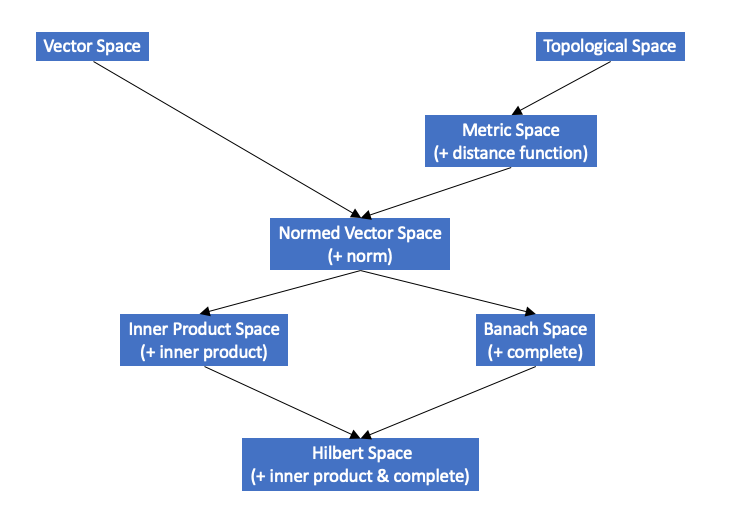
\includegraphics[width=0.8\textwidth]{../../images/function_spaces.png}
   \caption{Map of function spaces.}
   \label{fig:function_spaces}
\end{figure}

\begin{center}
\begin{tabular}{Sc|Sc|Sc}
    Space & Norm & Inner product \\
    \hline
    $C(M)$ & $ \displaystyle ||v||_C = \sup_{x \in M} |v(x)| $ & X \\
    \hline
    $C^k(M)$ & $\begin{aligned} &||v||_{C^k} = \max_{|\alpha| \le k} ||D^\alpha v||_C \\ &|v|_{C^k}=\max_{|\alpha| = k} ||D^\alpha v||_C \end{aligned}$ & X \\
    \hline
    $L_p(\Omega)$ & $ \displaystyle ||v||_{L_p} = \left ( \int_\Omega |v|^p \, dx \right)^{1/p} $ & X \\
    \hline
    $L_2(\Omega)$ & $ \displaystyle ||v||_{L_2} = \left ( \int_\Omega |v|^2 \, dx \right)^{1/2} $ & $ \displaystyle (v,w) = \int_\Omega vw^* \, dx $ \\
    \hline
    $H^k(\Omega)$ & $ \begin{aligned} &||v||_k = \left ( \sum_{|\alpha| \le k} ||D^\alpha v||^2 \right )^{1/2} \\ &|v|_k = \left ( \sum_{|\alpha| = k} ||D^\alpha v||^2 \right )^{1/2} \end{aligned}$ & $ \displaystyle (v,w)_k = \sum_{|\alpha \le k|} (D^\alpha v, D^\alpha w) $
\end{tabular}
\end{center}

\end{document}